\documentclass[11pt]{article}

\usepackage[portuguese]{babel}
\usepackage[a4paper,top=2cm,bottom=2cm,left=3cm,right=3cm,marginparwidth=1.75cm]{geometry}
\usepackage{amsmath}
\usepackage{graphicx}
\usepackage{float}
\usepackage[colorlinks=true, allcolors=blue]{hyperref}
\usepackage{listings}
\usepackage{hyphenat}
\usepackage{xcolor}

\title{\textbf{Projeto de Pesagem Automatizada de Gado (Sem título)}}
\author{
    Renan da Silva Oliveira Andrade (\texttt{renan.silva3@pucpr.edu.br})\\
    Ricardo Lucas Kucek (\texttt{ricardo.kucek@pucpr.edu.br})\\
    Pedro Senes Velloso Ribeiro (\texttt{pedro.senes@pucpr.edu.br})\\ 
    Riscala Miguel Fadel Neto (\texttt{riscala.neto@pucpr.edu.br})\\ Victor Valerio Fadel (\texttt{victor.fadel@pucpr.edu.br})
}

\begin{document}
\maketitle

\section{Descrição do contexto}

Em propriedades rurais, o controle de pesagem do corpo pecuário é indispensável para a manutenção da qualidade de vida dos animais. Controlar o peso dos bovinos/equinos ou quaisquer outros animais infere avaliar o desempenho em relação ao ganho de peso dos mesmos, algo de extrema importância para a pecuária comercial, pois impacta diretamente em sua produtividade e na lucratividade.

O controle de pesagem permite avaliar e ajustar a distribuição alimentar dos animais, garantindo que estes se desenvolvam de forma saudável. Em propriedades que trabalham com equinos, como haras e fazendas de criação, a pesagem auxilia na divisão correta da alimentação, suplementos e medicações, evitando sub ou sobrepeso, o que pode comprometer a saúde e a performance destes animais.

Além disso, o controle periódico do peso pode indicar animais que perderam peso de forma mais acentuada que o usual, fator este que pode alertar os criadores e cuidadores sobre possíveis doenças e evitar a piora do animal ou a possível disseminação da doença entre os demais animais, permitindo uma intervenção precoce e um manejo sanitário mais eficiente.

Em suma, o controle de pesagem dos animais nas propriedades rurais reflete-se diretamente no controle da qualidade da vida animal e na rentabilidade em propriedades rurais de cunho comercial.

\section{Problemática}
A pesagem manual de animais em propriedades rurais apresenta desafios como a necessidade de mão de obra especializada,
o estresse causado aos animais e a possibilidade de erros humanos na coleta e registro dos dados.
Além disso, a falta de um controle de pesagem eficiente pode resultar em uma nutrição não otimizada,
comprometendo o crescimento e a saúde dos animais. Na pecuária comercial,
a ausência de um monitoramento preciso do peso impacta diretamente na produtividade e na lucratividade,
dificultando a identificação precoce de doenças e problemas nutricionais.
A implementação de um sistema automatizado de pesagem torna-se essencial para garantir um manejo mais eficiente e melhorar a qualidade de vida dos animais.

\section{Motivação}
Apesar da importância do controle de peso dos animais, a pesagem na maioria das propriedades rurais de médio e pequeno porte ainda é realizada manualmente, exigindo mão de obra especializada para o registro de dados e o manejo dos animais. Esse método pode tornar a saúde dos animais vulnerável a possíveis erros no manejo e no controle das informações. Diante disso, um sistema automatizado de pesagem e registro de dados aumentaria a eficiência dos recursos humanos e financeiros da propriedade, além de evitar problemas como a falta de confiabilidade dos dados, decorrente de erros humanos, e a necessidade de um meio físico para o armazenamento das informações.

\section{Proposta}
O controle de pesagem dos animais em propriedades rurais é essencial para garantir a saúde e o qualidade adequada dos bovinos, equinos e outros animais. A pesagem manual feita com mão de obra humana apresenta desafios, como a necessidade de mão de obra especializada, estresse nos animais e possíveis erros humanos. Assim, um sistema automatizado de pesagem se torna uma solução eficiente para melhorar o manejo e a produtividade de criadouros.

\subsection{Descrição do Sistema}
O sistema proposto utilizará tecnologia NFC (\textit{Near Field Communication}) para a identificação individual dos animais e um mecanismo de controle para garantir que apenas um animal seja pesado por vez. Cada animal usará um colar equipado com uma tag NFC única, permitindo sua identificação automática no momento da pesagem.

\subsection{Mecanismo de Pesagem}
O sistema contará com balanças eletrônicas cercadas por dois portões automatizados, que se fecharão assim que um animal entrar na balança. Antes da medição do peso, serão realizadas as seguintes verificações:

\begin{itemize}
    \item Verificação da tag NFC: O sistema identifica o animal e confirma a presença de apenas uma tag no momento da pesagem.
    \item Verificação do peso: O peso detectado é comparado com um peso limite para garantir que corresponda a o peso de um único animal.
\end{itemize}

Se ambas as verificações forem aprovadas, o peso do animal será medido e registrado.

\subsection{Armazenamento e Acesso aos Dados}
As informações de cada pesagem, incluindo a tag NFC do animal e seu peso, serão armazenadas em um banco de dados MySQL, e o acesso dos dados será feito por meio de uma aplicação web desenvolvida em Flask, que permitirá que os usuários:

\begin{itemize}
    \item Visualizem o peso individual de cada animal;
    \item Ordenem a lista de animais pelo peso;
    \item Visualizem a média de peso do rebanho;
    \item Receber alertas automáticos caso haja variações e / ou anomalias no peso dos animais.
\end{itemize}

\subsection{Suporte de navegação com Chat IA}
A aplicação contará com um chat com inteligência artificial de linguagem natural, permitindo que os usuários interajam com o sistema de maneira intuitiva. Os usuários poderão acessar todas as informações do site por meio do chat, que interpretará a pergunta e os levará para a informação demandada sem a necessidade de um conhecimento de computadores prévio.

O sistema de pesagem automática proporcionará um monitoramento eficiente e automatizado da saúde e do desenvolvimento dos animais, reduzindo erros, otimizando a nutrição e garantindo um manejo mais inteligente e produtivo na pecuária.

\section{Tecnologias envolvidas}
\section{Resultados esperados}
\section{Cronograma}

\begin{figure}[H]
    \centering
    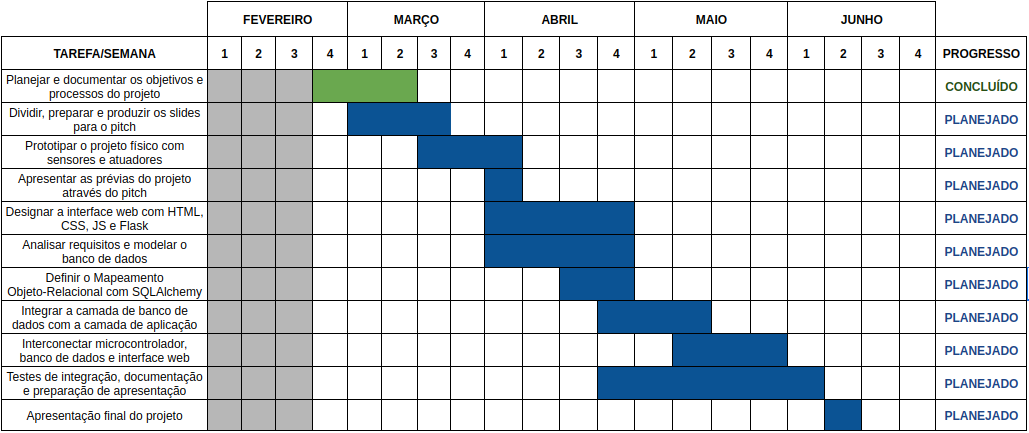
\includegraphics[width=0.9\linewidth]{cronograma.png}
    \caption{Cronograma}
\end{figure}

\bibliographystyle{apalike}
\bibliography{sample}

\end{document}
